\section{Community Evaluation: Synthetic network}
\label{eval}
We evaluate the performance of the proposed multilayer community detection algorithms \textbf{GN-$Q_M$} and \textbf{Louvain-$Q_M$} in a
controlled environment. First we present the experimental setup explaining the generation of synthetic multilayer network
with ground truth communities and the evaluation metric. Next, we present the competing baseline algorithms and
finally, we exhibit the elegance of the proposed algorithms over baselines from different perspectives.
% Additionally, we also discuss about the scalability \& adaptability of our algorithm for larger and more
% complicated network [BM: do we really want it?] structures.

\subsection{Experimental setup}
We generate the synthetic two layer networks ($\mathcal{G} = \{\{L_1, L_2\}, \{L_{12}\}\}$) with planted communities
following the model proposed in section~\ref{syn_gen}.
We fix the number of nodes $|V_i|$ in each layer $L_i$ at $100$ with maximum degree $k^{i}_{max}=10$ \& average
degree $\langle k_i\rangle=6$. The power-law exponents for degree distribution ($\gamma_i$) and community size distribution ($\beta_i$)
for each layer are fixed at 2 and 1 respectively.
The other model parameters ($\mu$, $\alpha$, $p$ \& $d$) are regulated and adjusted according to the requirement.
We apply the normalized mutual information (NMI)~\cite{danon2005comparing} as the yardstick
to quantify the similarity between the detected and ground truth communities.
% Suppose, $N$ is the number of nodes in the entire multilayer network,
% $w_1, w_2, \dots, w_W$ are the sets of nodes (all layers combined) contained in the
% detected $W$ communities and $r_1, r_2, \dots, r_R$ are the sets of nodes (all layers combined) contained in the
% total $R$ ground truth communities.
% Then NMI, of this two sets of communities can be calculated as
%
% \begin{equation}
%  NMI = \frac{\sum_{k=1}^{W} \sum_{j=1}^R \frac{\left \vert w_k \cap r_j \right \vert}{N} \log \frac{N \left \vert w_k \cap r_j \right \vert}
%  {\left \vert w_k \right \vert \left \vert r_j \right \vert}} {[(-\sum_{k=1}^W\frac{\left \vert w_k \right \vert}{N}
%  \log \frac{ \left \vert w_k \right \vert}{N} ) + (-\sum_{j=1}^R \frac{\left \vert r_j \right \vert}{N}
%  \log \frac{ \left \vert r_j \right \vert}{N})]/2}
% \end{equation}
%
%$NMI$ attains higher value if the ground truth and detected communities exhibit good agreement.
The synthetic network contains $30$
single layer (\& no cross layer) ground truth communities when $\alpha = 0$ and $15$
cross layer (\& no single layer) ground truth communities when $\alpha = 1$.

%If both match completely, we have a maximum NMI value of 1, whereas if the obtained and ground truth partitions are totally independent of one another, we have a minimum value of 0. Such kind of testing is widely used by other researchers in the community detection field[CITE?].


% \begin{figure}
% \centering
% 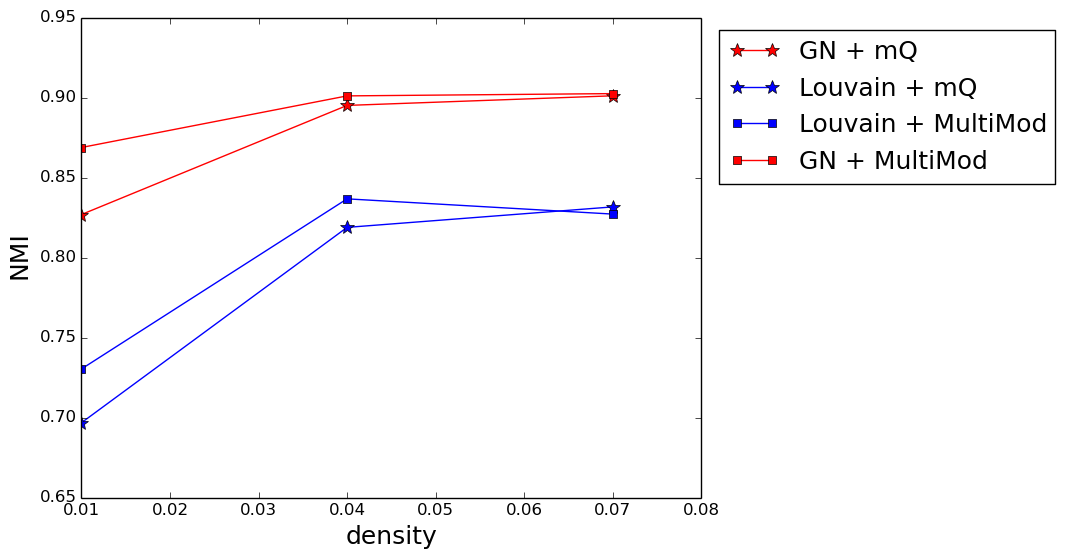
\includegraphics[width=3.5in]{./images/NMI_D_P0_4_A0_6_MU0_05.png}
% \vspace{-0.1in}
% \caption{NMI of obtained and ground truth communities various $d$ values for $p=0.4$, $\alpha=0.6$, $\mu=0.05$}
% \vspace{-0.1in}
% \label{nmi1}
% \end{figure}
\subsection{Competing algorithms}
%As we mentioned before, any single layer community detection algorithm which maximizes modularity or a similar metric can be used as
%our algorithm. In this paper, we choose Girvan-Newman~\cite{newman2004fast} (GN) and Louvain~\cite{blondel2008fast} as our
%single layer algorithms on top of which we use our $Q_M$ metric. We compare this two methods with the following two types of
%baseline methods.
% [BM: Use the following naming convention; \textbf{GN-$Q_M$}, \textbf{Louvain-$Q_M$}, \textbf{GN-$mQ$} and
% \textbf{Louvain-$mQ$} etc]
We introduce the following three classes of competing algorithms to evaluate the
performance of \textbf{GN-$Q_M$} and \textbf{Louvain-$Q_M$}.

\subsubsection{Baselines with $mQ$} We induce the multilayer modularity $mQ$ proposed in~\cite{medical_paper} with the standard
 Girvan-Newman and Louvain algorithms~\cite{newman2004finding},~\cite{blondel2008fast}. We refer these baseline algorithms 
 as \textbf{GN-$mQ$} and \textbf{Louvain-$mQ$} respectively.

\subsubsection{Merging based baselines} We apply standard Louvain algorithm~\cite{blondel2008fast} to
 detect communities at the individual layers and then attempt to merge those communities across the layers.
 We merge one top layer community $C_T$ with one bottom layer community $C_B$ with which it is maximally connected 
 if the connection density between them is above a threshold\footnote{Merging is performed if the ratio of the number of coupling links 
 between $C_T$ \& $C_B$ and the total number of 
 coupling links connected with $C_T$ \& $C_B$ is at least $Th$. We vary $Th$ from $0.1$ to $1.0$ and report the best obtained result.}; 
 otherwise keep $C_T$ and $C_B$ as a single layer community.

\subsubsection{State-of-the-art algorithms} We implement `MetaFac'~\cite{metafac} and `CompMod'~\cite{CompMod} as state of the art multilayer community
detection algorithms, already introduced in section~\ref{syn_evalu}.

\begin{figure}
\begin{center}
\subfigure[Varying $d$ values for $p=0.4$, $\alpha=0.6$, $\mu=0.05$ for $mQ$ based baselines
]{\label{nmi1}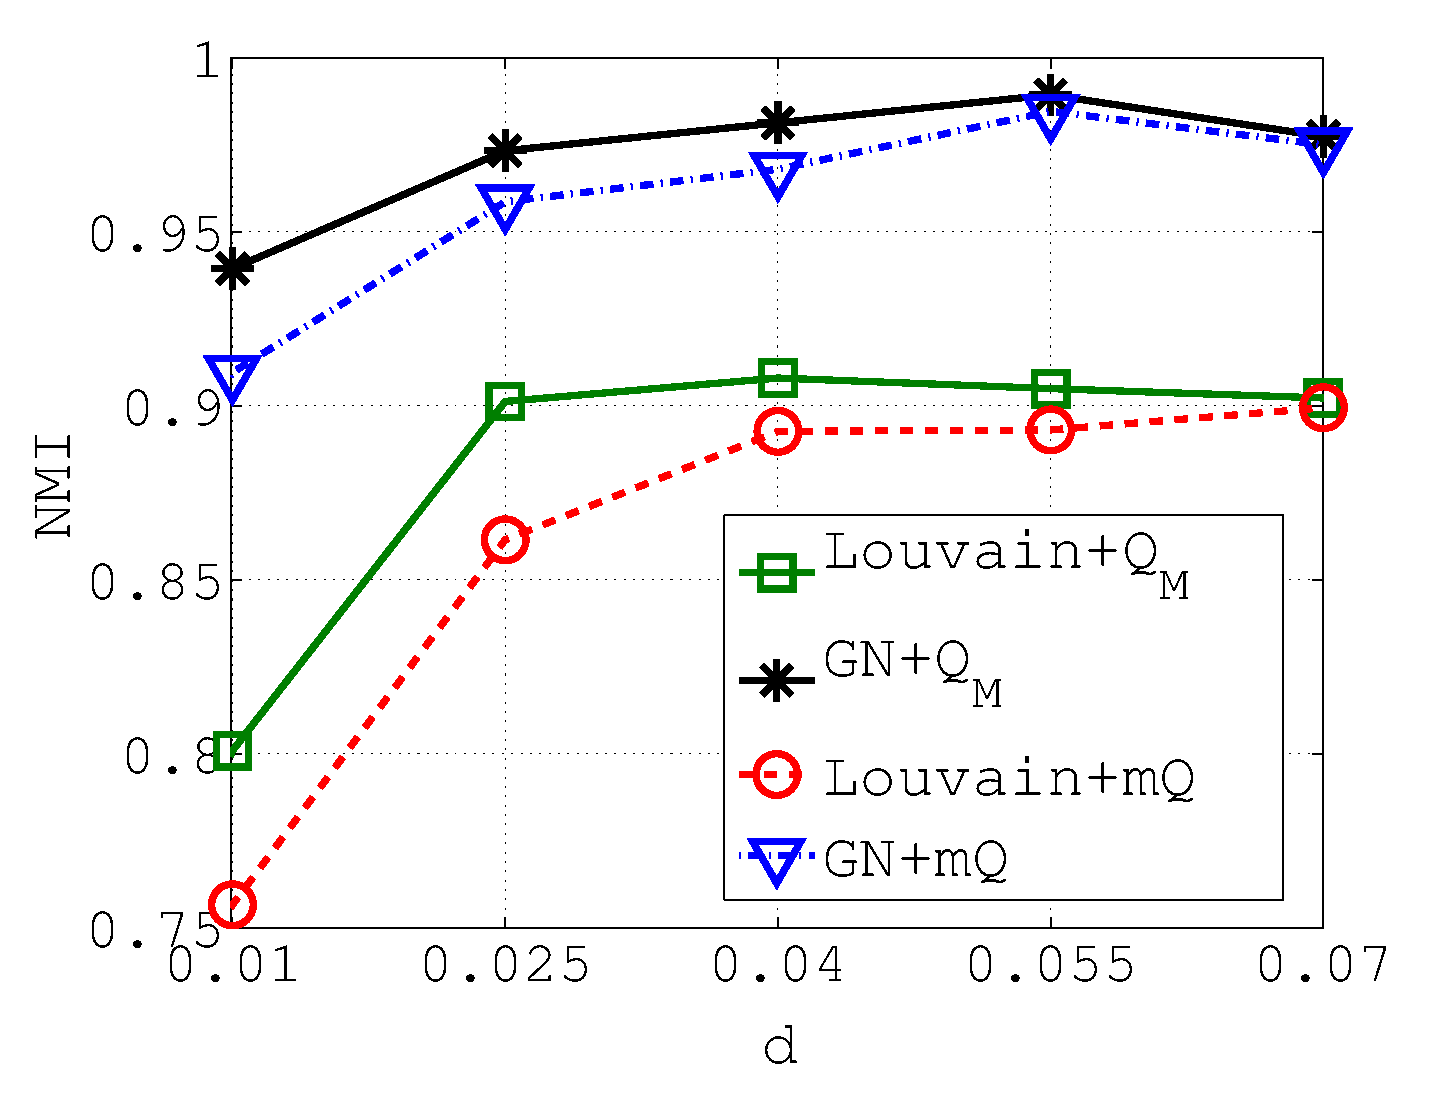
\includegraphics[angle=0,scale=.17]{./images/NMI_density_mQ_QM.pdf}}
\subfigure[Varying $d$ values for $p=0.4$, $\alpha=0.6$, $\mu=0.05$ for merging based baselines
]{\label{nmi1_1}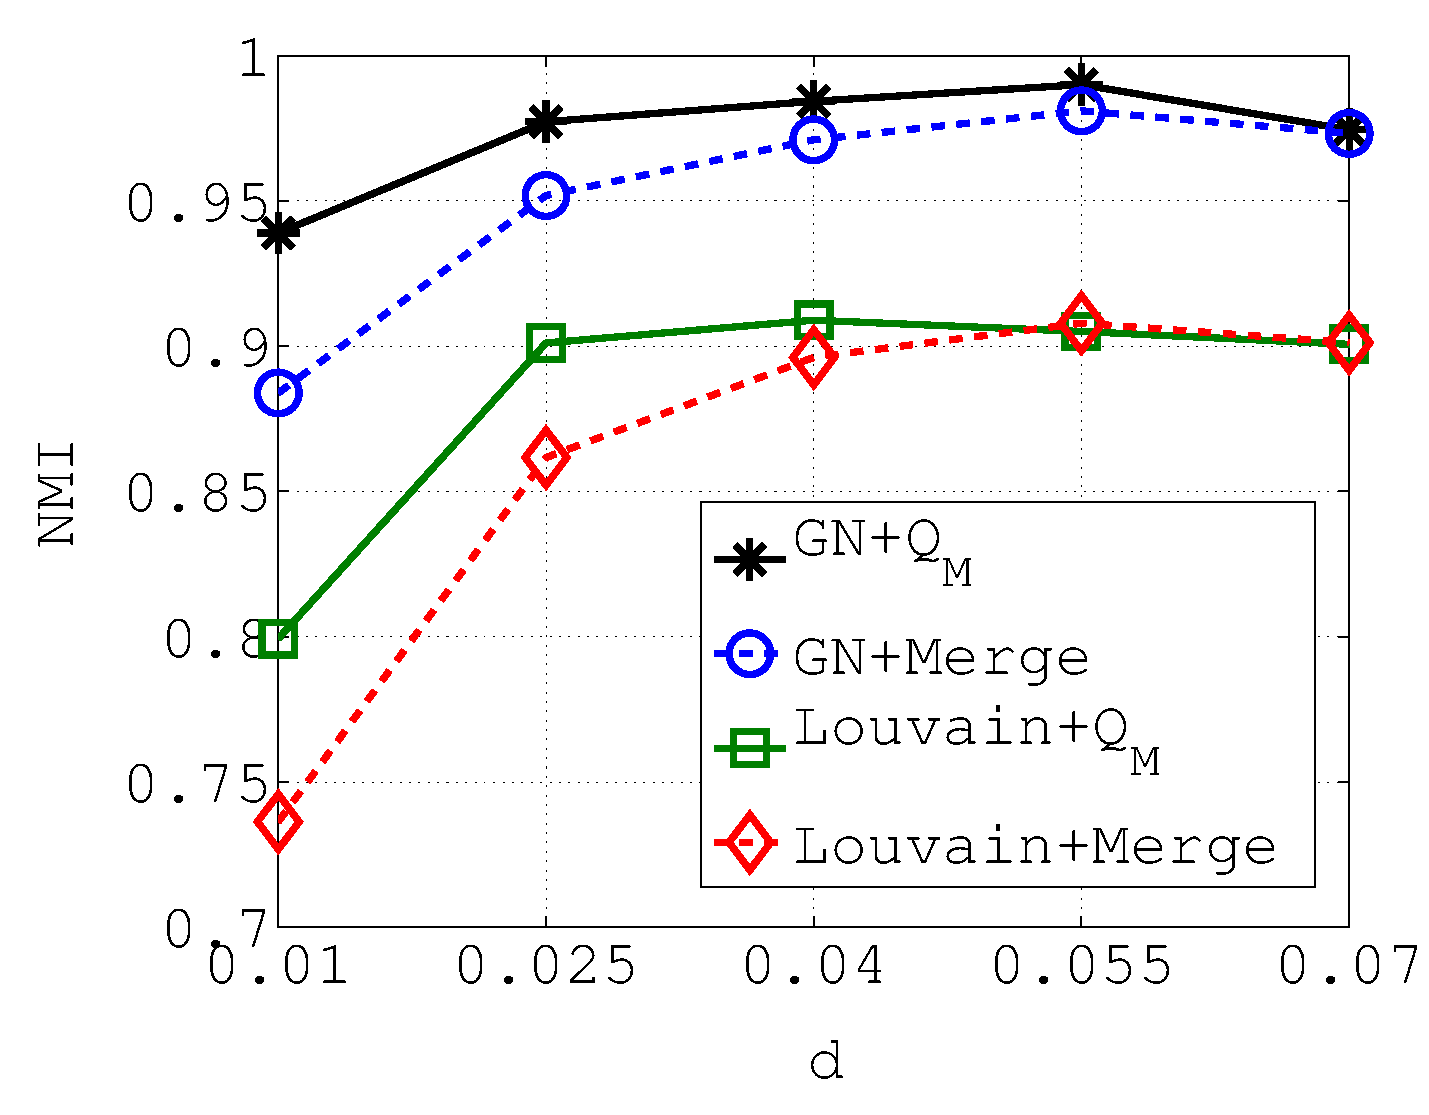
\includegraphics[angle=0,scale=.17]{./images/NMI_density_merge_QM.pdf}}
\end{center}
\vspace{-0.24in}
\caption{NMI of obtained and ground truth communities for various $d$ values.}
\vspace{-0.22in}
\label{nmi00}
\end{figure}



% \begin{figure}
% \begin{center}
% \subfigure[Precision
% ]{\label{reco1}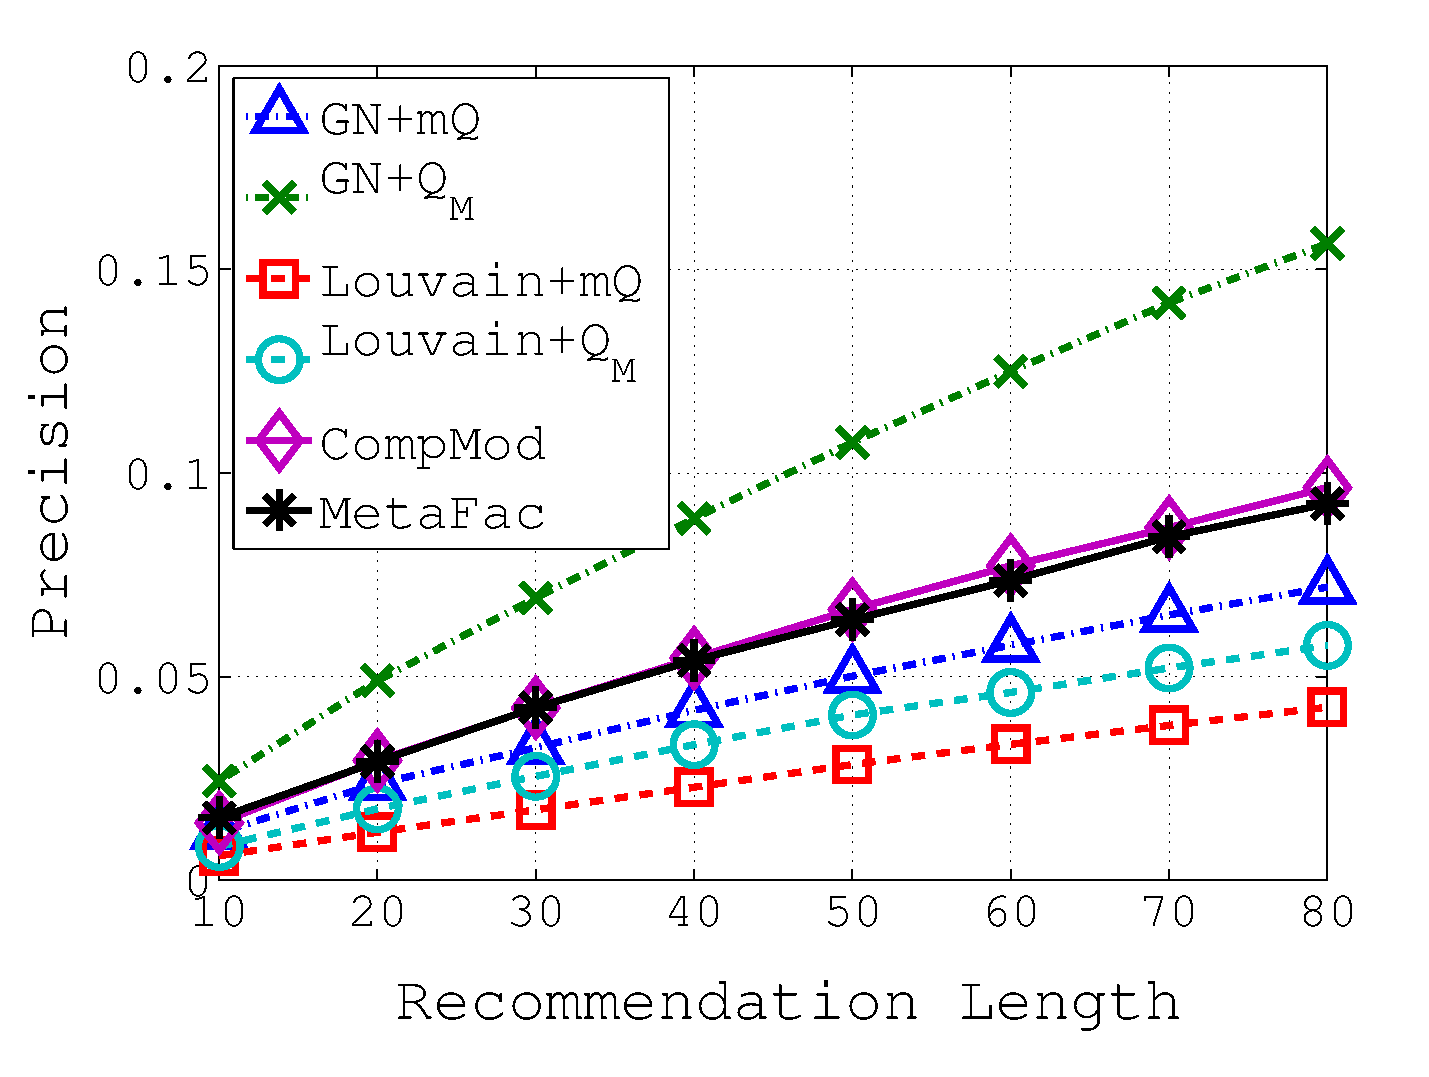
\includegraphics[angle=0,scale=.18]{./images/Intersection_Reco_march21_square.pdf}}
% \subfigure[F1 Score
% ]{\label{reco0}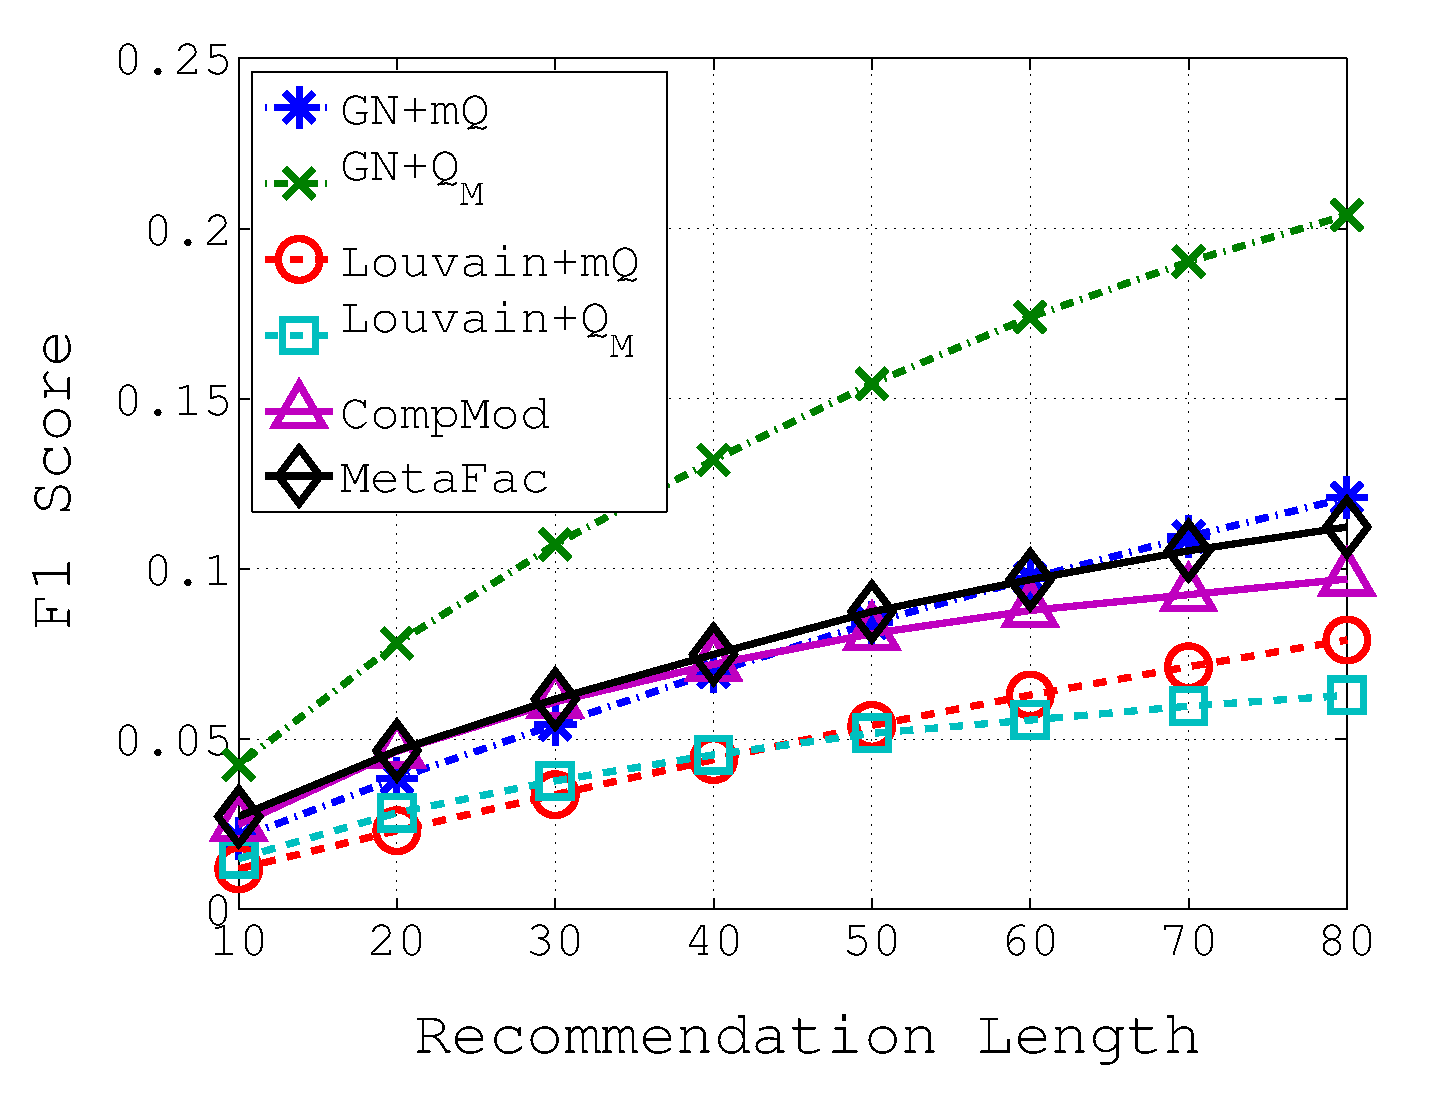
\includegraphics[angle=0,scale=.18]{./images/F1_Reco_march21_square.pdf}}
% \end{center}
% \vspace{-0.3in}
% \caption{Precision \& F1 Score for communities obtained from different algorithms for various recommendation lengths}
% \vspace{-0.22in}
% \label{reco}
% \end{figure}

\subsection{Evaluation}
\subsubsection{Comparison with baselines with $mQ$}
The proposed \textbf{GN-$Q_M$} and \textbf{Louvain-$Q_M$} algorithms perform quite closely with their respective benchmark 
\textbf{GN-$mQ$} and
\textbf{Louvain-$mQ$}  However, the improvement gets manifested when we reduce the density
of coupling links $d$. In Fig.~\ref{nmi1}, we observe that \textbf{GN-$Q_M$} and \textbf{Louvain-$Q_M$} outperform the baselines in the
lower link density regime. This comes from the fact that the modularity $mQ$ fails to reflect the cohesiveness
of multilayer communities for low $d$ values, as explained in Fig.~\ref{cross_multi}.

\subsubsection{Comparison with merging based baselines}
This baseline
%\footnote{For each configuration, we vary the threshold of merging and depict the one giving the best NMI.} 
performs pretty close to aforesaid \textbf{GN-$mQ$} and \textbf{Louvain-$mQ$}  since here
also we optimize the
modularities at top, bottom and bipartite layers separately. Evidently, the proposed \textbf{GN-$Q_M$} and \textbf{Louvain-$Q_M$} 
algorithms outperform
this baseline in the low coupling link density ($d$) regimes (see Fig.~\ref{nmi1_1}).

%Hence, as expected, the merging based baselines perform quite closely with the corresponding
% and fails to reflect the cohesiveness of multilayer communities in $d$, as explained in Fig.~\ref{single0}. The higher NMI of \textbf{GN-$Q_M$} and Louvain-$Q_M$
% manifests the elegance of the proposed modularity index $Q_M$.


\subsubsection{Comparison with state-of-the-art algorithms}
% \begin{figure}
% \centering
% 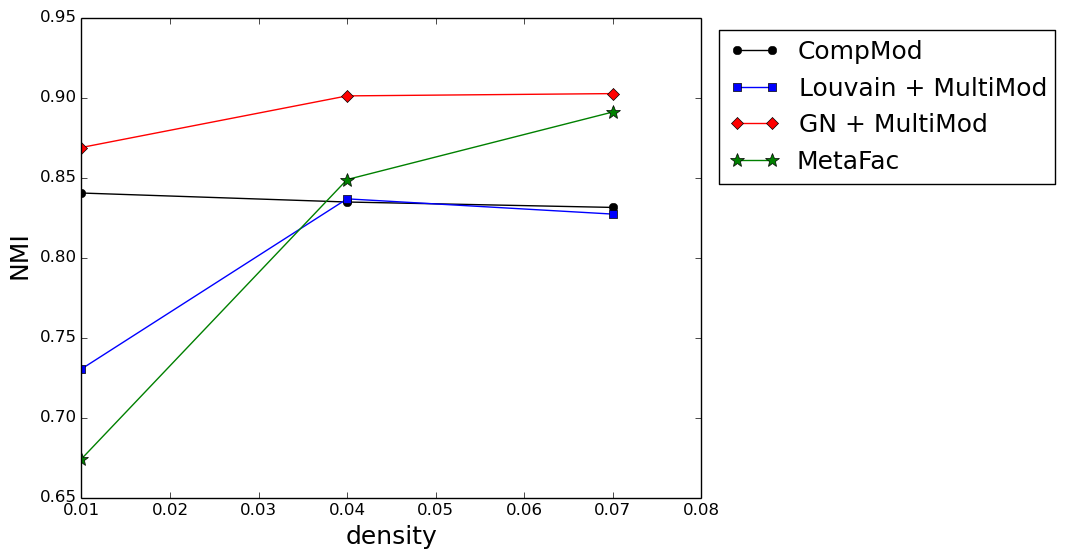
\includegraphics[width=3.5in]{./images/NMI_D2_P0_4_A0_6_MU0_05.png}
% \vspace{-0.1in}
% \caption{NMI of obtained (nmi for mQ and nmia for $Q_{adapt}$) and ground truth communities for p=0.9}
% \vspace{-0.1in}
% \label{nmi}
% \end{figure}

\textbf{(a) Effect of $\alpha$:} The model parameter $\alpha$ regulates the proportion of ground truth cross layer
(against single layer) communities in the
 synthetic multilayer network. In Fig.~\ref{nmi2}, we observe that \textbf{GN-$Q_M$} and \textbf{Louvain-$Q_M$} do not exhibit high
 sensitivity with $\alpha$; this points to the
 fact that performance of these two algorithms (specially GN-$Q_M$) does not depend on the proportion of single layer
 and cross layer communities present in the network. However, the performance of $MetaFac$ monotonically improves
 with increasing $\alpha$ whereas $CompMod$
exhibits the opposite behaviour. In fact, $MetaFac$ algorithm is intrinsically biased towards detecting cross layer
communities whereas
 $CompMod$ is more suitable for detecting single layer communities.
\textbf{(b) Effect of $p$:}  Model parameter $p$ realizes the cohesiveness of the coupling links in the apriori cross layer communities.
We observe (see Fig.~\ref{nmi4}) that our algorithms outperform $MetaFac$ and $CompMod$ in the presence of moderate to cohesive 
cross layer communities (say $p>0.3$). However, for $p<0.3$ $CompMod$ performs relatively better due to the degradation of
the cross layer communities, since $CompMod$ intrinsically favors the single layer communities.

\begin{figure}
\begin{center}
\subfigure[Varying $\alpha$ values for $p=0.8$, $\mu=0.4$ and $d=0.04$
]{\label{nmi2}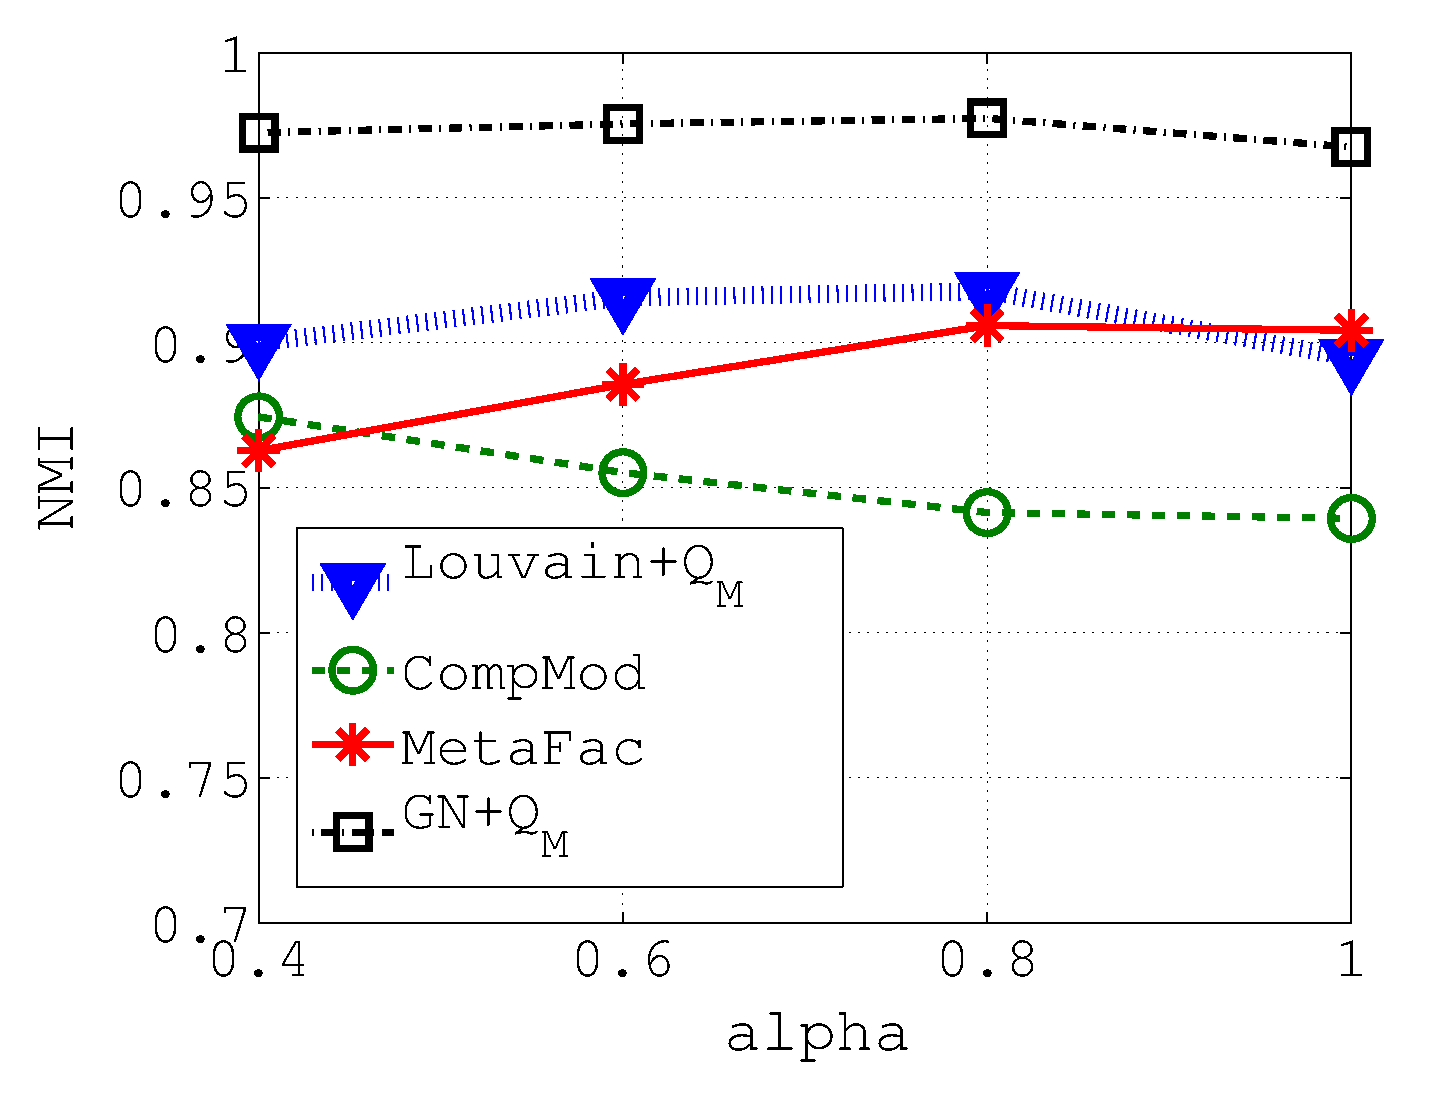
\includegraphics[angle=0,scale=.17]{./images/NMI_alpha_QM.pdf}}
% \subfigure[Varying $\mu$ values for $p=0.8$, $\alpha=0.6$ and $d=0.04$
% ]{\label{nmi3}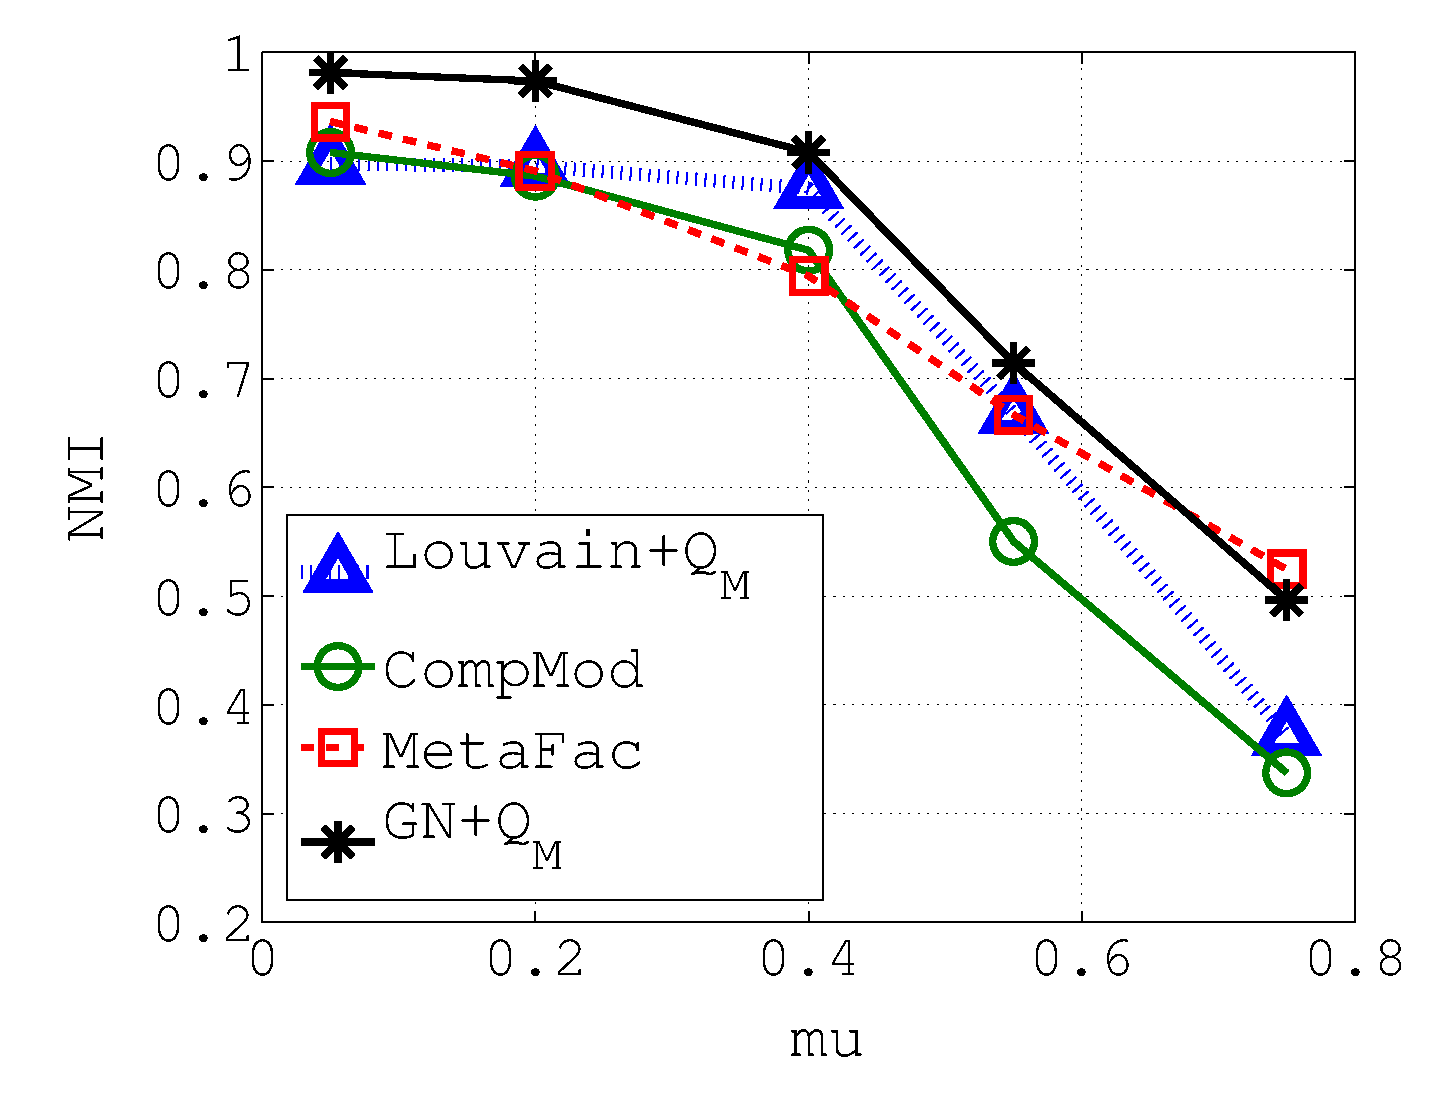
\includegraphics[angle=0,scale=.21]{./images/NMI_mu_QM.pdf}}
\subfigure[Varying $p$ values for $\mu=0.4$, $\alpha=0.6$ and $d=0.04$
]{\label{nmi4}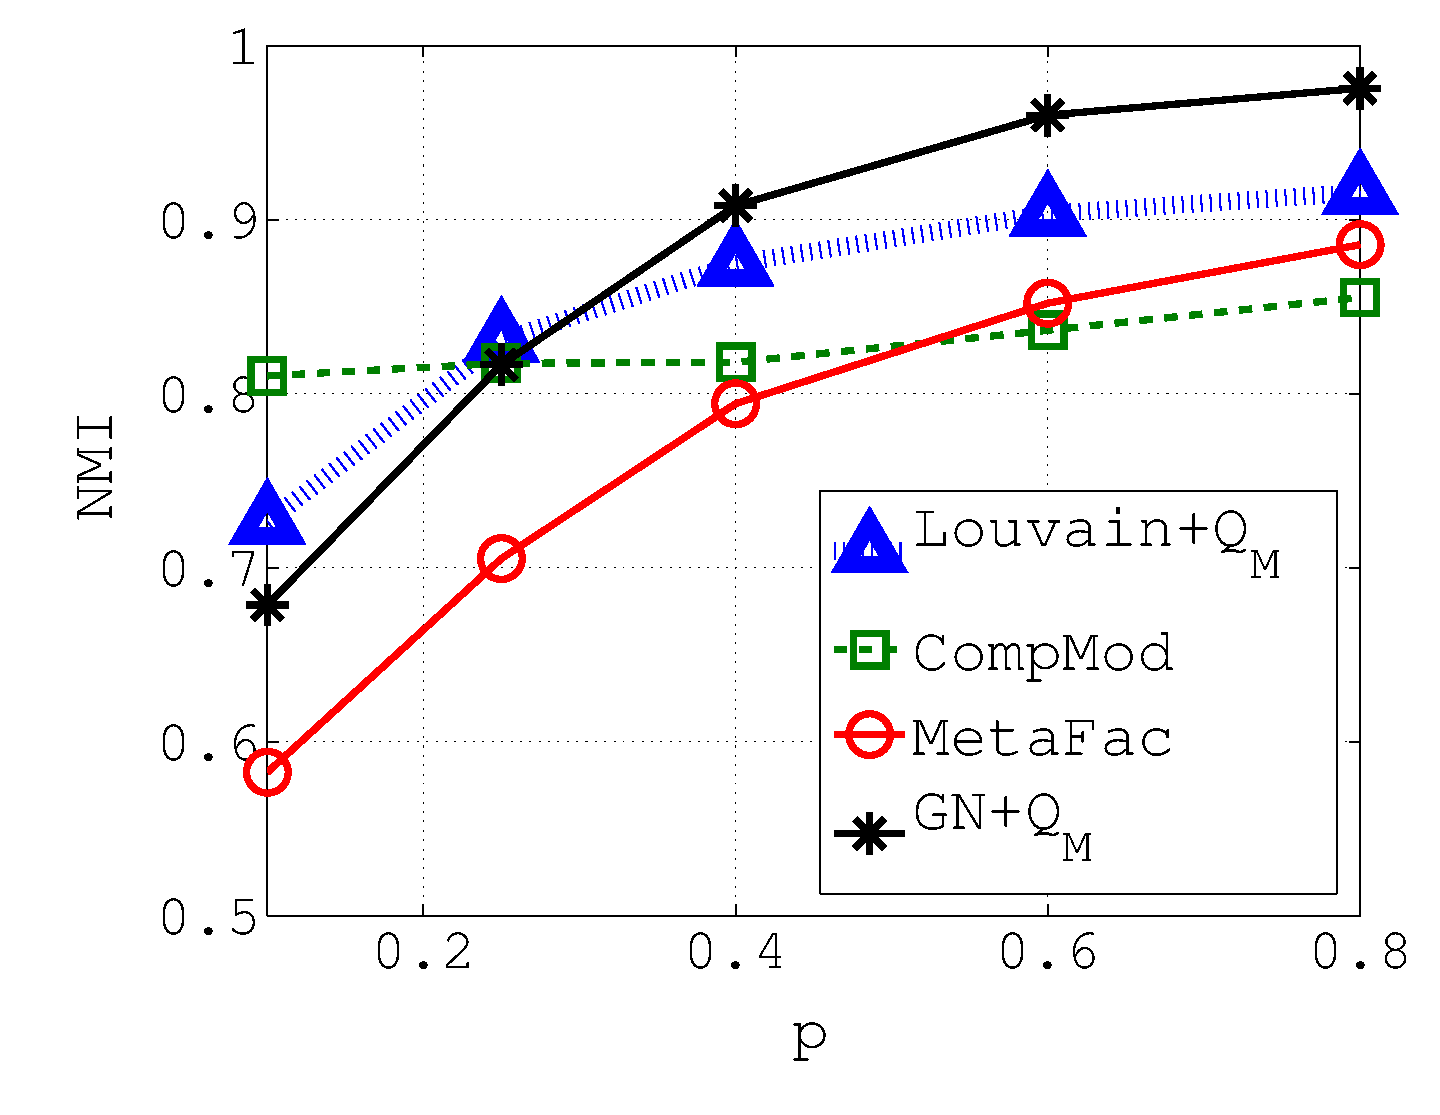
\includegraphics[angle=0,scale=.17]{./images/NMI_p_QM.pdf}}.
\end{center}
\vspace{-0.23in}
\caption{NMI of obtained and ground truth communities for various $\alpha$ \& $p$ values.}
\vspace{-0.25in}
\label{nmi11}
\end{figure}


% \begin{figure}
% \centering
% 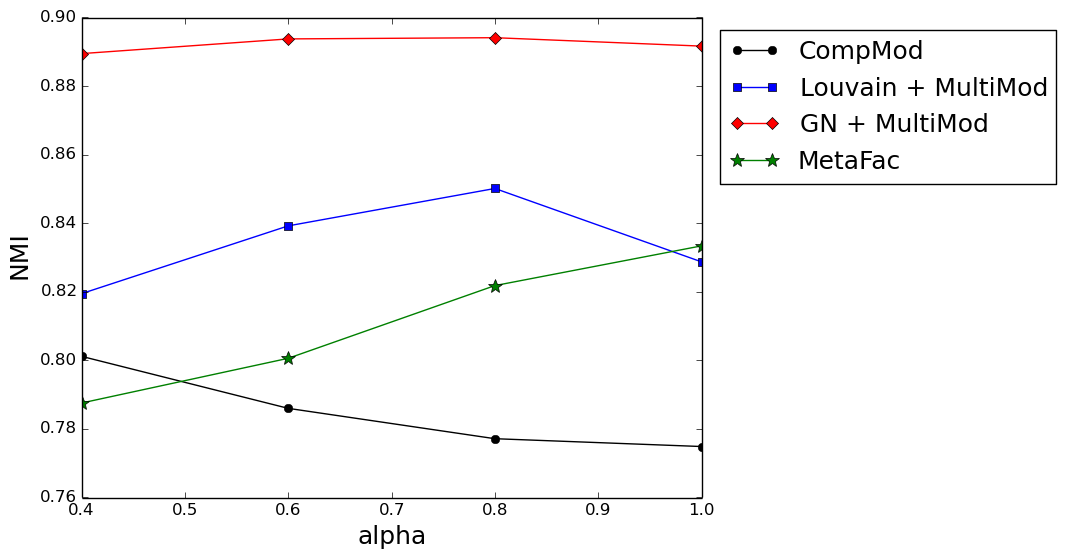
\includegraphics[width=3.5in]{./images/NMI_A_P0_8_MU0_4_D0_04.png}
% \vspace{-0.1in}
% \caption{NMI of obtained and ground truth communities with various $\alpha$ values for $p=0.8$, $\mu=0.4$ and $d=0.04$}
% \vspace{-0.1in}
% \label{nmi2}
% \end{figure}

% \item Effect of $\mu$: $\mu$ is the LFR parameter which decides the cohesivity of the single layer communities in the
% first step of synthetic network generation; increasing $\mu$ degrades the community cohesivity.
% We observe decreasing NMI for all the algorithms with increasing $\mu$ in Fig.~\ref{nmi3}.
% Nevertheless, \textbf{GN-$Q_M$} performs marginally better than competing algorithms.
% This is possibly because higher $\mu$ indicates poor cohesiveness; hence, poor quality of ground
% truth communities.



% \begin{figure}
% \centering
% 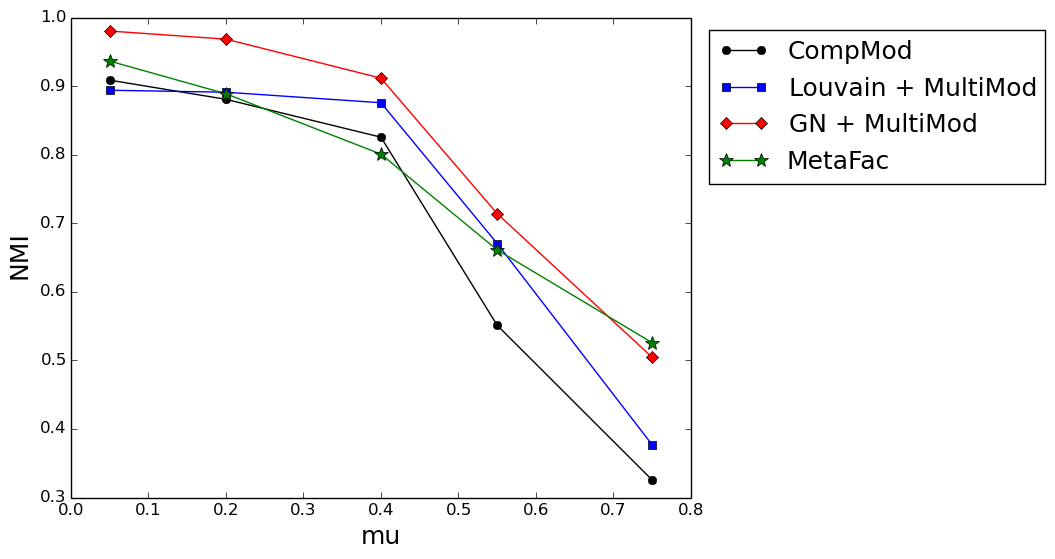
\includegraphics[width=3.5in]{./images/NMI_MU_P0_4_A0_6_D0_04.png}
% \vspace{-0.1in}
% \caption{NMI of obtained and ground truth communities with various $\mu$ values for $p=0.8$, $\alpha=0.6$ and $d=0.04$}
% \vspace{-0.1in}
% \label{nmi3}
% \end{figure}

% \begin{figure}
% \centering
% 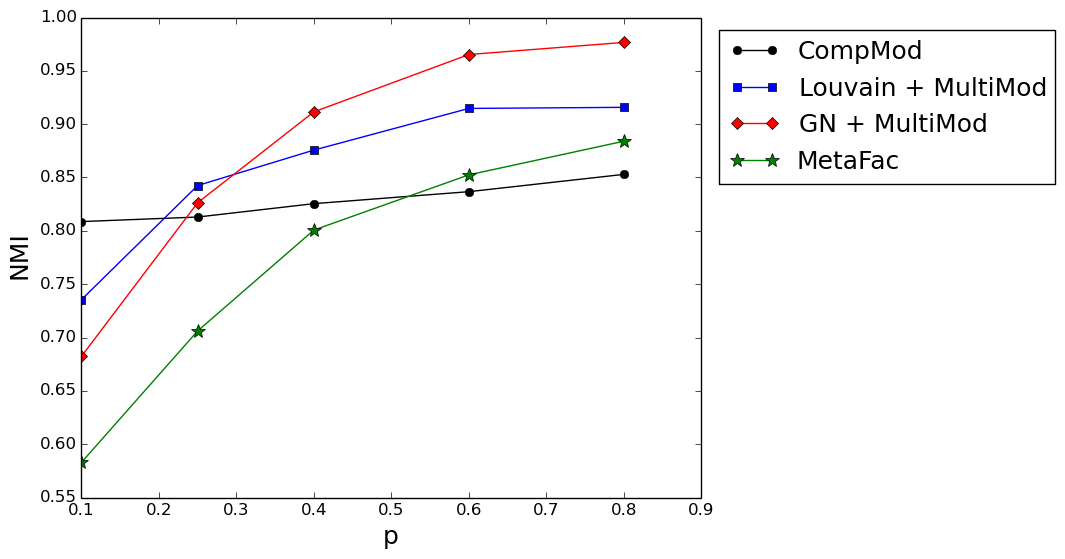
\includegraphics[width=3.5in]{./images/NMI_P_A0_6_MU0_4_D0_04.png}
% \vspace{-0.1in}
% \caption{NMI of obtained and ground truth communities with various $p$ values for $\mu=0.4$, $\alpha=0.6$ and $d=0.04$}
% \vspace{-0.1in}
% \label{nmi4}
% \end{figure}


%[BM: check. dropped $\mu$]
In a nutshell, we claim that (a) the proposed algorithms show pretty balanced behaviour across different range of model
parameters ($d$, $p$ etc) and (b) importantly, they can
simultaneously detect both single layer and cross layer communities without any specific bias towards anyone of 
them (invariant to $\alpha$).
Though \textbf{GN-$Q_M$} and \textbf{Louvain-$Q_M$} perform relatively poorly in the lower $p$ regions, notably, they never rank as the
worst in the batch. $CompMod$ performs decently in lower $p$ regions due to its intrinsic bias towards cross layer communities,
where $MetaFac$ fails miserably.

%R[BM: In the entire paper, replace cross layer link as coupling link.]

% \subsection{Comparison with baselines}
% Compare the results produced by different baselines on different synthetic networks with our algorithm's results. We
% may use different metrics like NMI, ARI, Purity etc. and their weighted versions \cite{metric} for comparisons. We
% need to also explain the reason of the success of our algorithm and modularity metric. The baseline algorithms can be the ones used in
% \cite{InfoCom} (CompMod~\cite{CompMod}, MetaFac~\cite{metafac}, NaiveSimp, Trans-C, Trans-JD),
% the algorithm InfoCom proposed in ~\cite{InfoCom} itself
% and the algorithm proposed in ~\cite{medical_paper}.\textcolor{red}{[SP: I have already received the code for CompMod~\cite{CompMod}. If
% Raphael can implement InfoCom~\cite{InfoCom} and MetaFac~\cite{metafac} (at least the MetaFac), it will be very helpful. Implementing others
% are relatively trivial.]}
%
% \subsection{Effect of varying Parameters}
% In this subsection, we apply the Newman-Girvan community detection algorithm with modularity replaced by $mQ$ and $Q_{adapt}$ on different
% synthetic networks generated with different parameters. This is done to analyze the impact of those parameters on the ground
% truth and obtained communities. In general, the communities obtained by maximizing $mQ$ and $Q_{adapt}$ are very similar
% irrespective of the synthetic network parameters.
%
% \begin{figure}
% \begin{center}
% \subfigure[Modularity of Ground Truth communities (Qt) and communities obtained using $mQ$ as a metric (Q) and
% using $Q_{adapt}$ as a metric (Qa) at p=0.9
% ]{\label{Q1}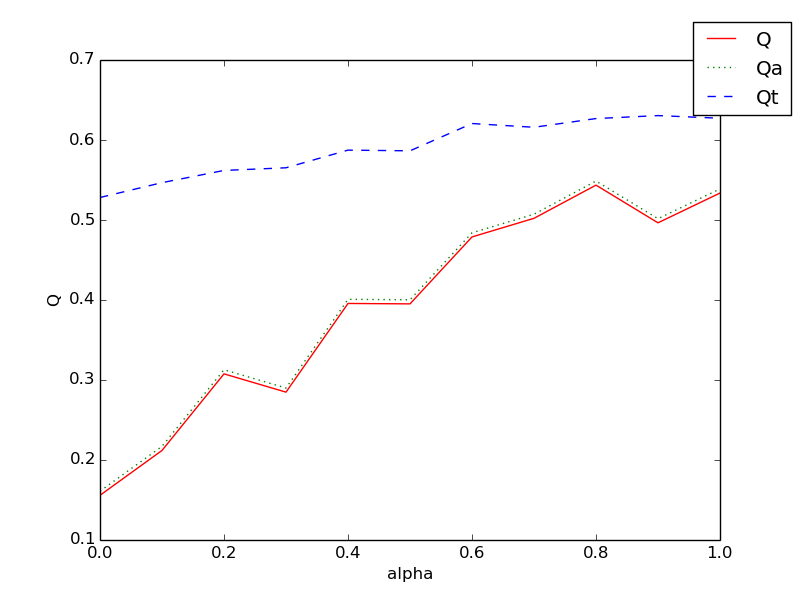
\includegraphics[angle=0,scale=.25]{./images/Q0_9.png}}
% \subfigure[Modularity of obtained communities using $mQ$ as a metric (Q) and
% using $Q_{adapt}$ as a metric (Qa) removing a fraction $g$ of cross community coupling edges at p=0.7.
% ]{\label{Q2}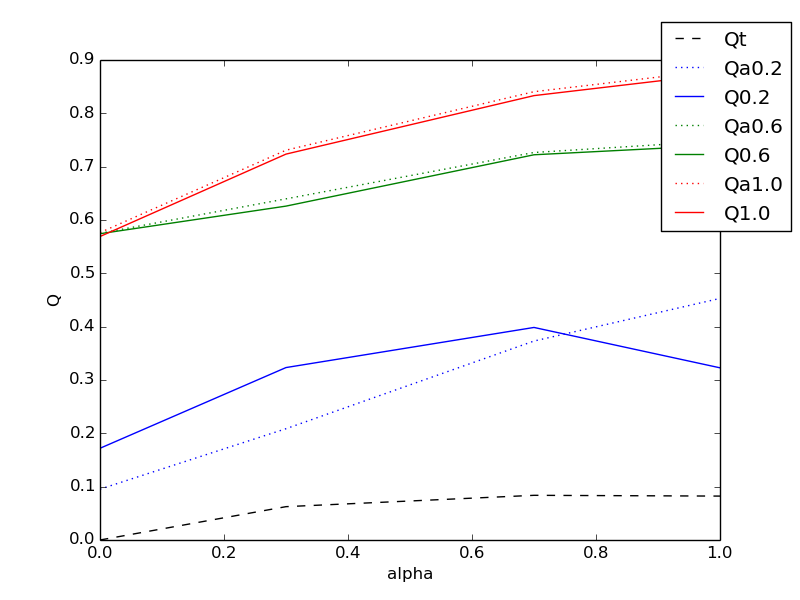
\includegraphics[angle=0,scale=.25]{./images/Q0_7_mp0_65.png}}
% \end{center}
% \vspace{-0.22in}
% \caption{Modularity of Ground Truth and obtained communities}
% \label{Q}
% \end{figure}
%
%
%
%
% \begin{enumerate}
%  \item \textbf{Effect of $p$ and $\alpha$ on modularity:} We observe that if $p$ is high i.e. most of the coupling edges are within
%  cross-layer communities, then modularity of the ground truth communities as well as obtained communities increase
%  with $\alpha$ (fraction of multilayer communities in ground truth)
%  (see Fig.~\ref{Q1}). This happens because high $\alpha$ implies that most of the ground-truth communities are multilayer and
%  high $p$ implies that most of the multilayer communities are of good quality. This two factors jointly help to increase the modularity
%  of the ground truth and obtained communities. The opposite occurs when $p$ is low i.e. modularity decreases with increasing $\alpha$ in
%  that case.\\
%  \item \textbf{Effect of deleting fraction of cross community coupling edges on modularity:} A disadvantage of our synthetic network
%  generation procedure is that we cannot fully control the number of coupling edges. The parameter $p$ just controls the fraction
%  of coupling edges within and outside the cross-layer communities. In general, the count of
%  cross community coupling edges is quite high with respect to the amount of single layer edges. This disrupts the cross-layer
%  community structure and lowers the modularity for ground truth and obtained communities.
%  If we remove a fraction $g$ of cross community coupling edges before running the community
%  detection algorithm, the modularity of the obtained communities improve (see Fig.~\ref{Q2}). The reason is intuitive - removing
%  cross community coupling edges essentially improves the quality of the cross-layer communities. The obtained communities even have higher
%  modularity than the ground truth communities.\\
%
% \begin{figure}
% \begin{center}
% \subfigure[CDF of different types of deleted edges while running Newman-Girvan algorithm with iterations for
% mixing parameter 0.05, p=0.7 and $\alpha$=0.7
% ]{\label{d1}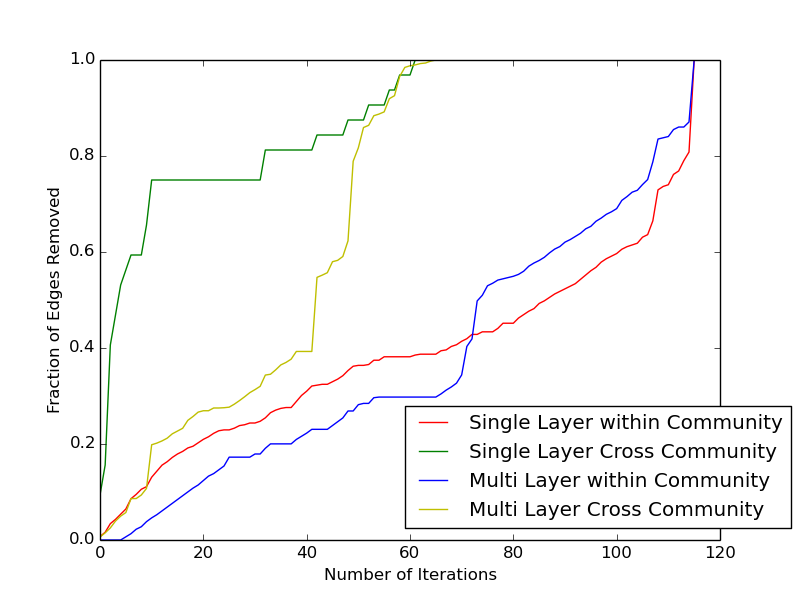
\includegraphics[angle=0,scale=.25]{./images/mp05_0_7_0_7_0_2.png}}
% \subfigure[CDF of different types of deleted edges while running Newman-Girvan algorithm with iterations for
% mixing parameter 0.65, p=0.7 and $\alpha$=0.7
% ]{\label{d2}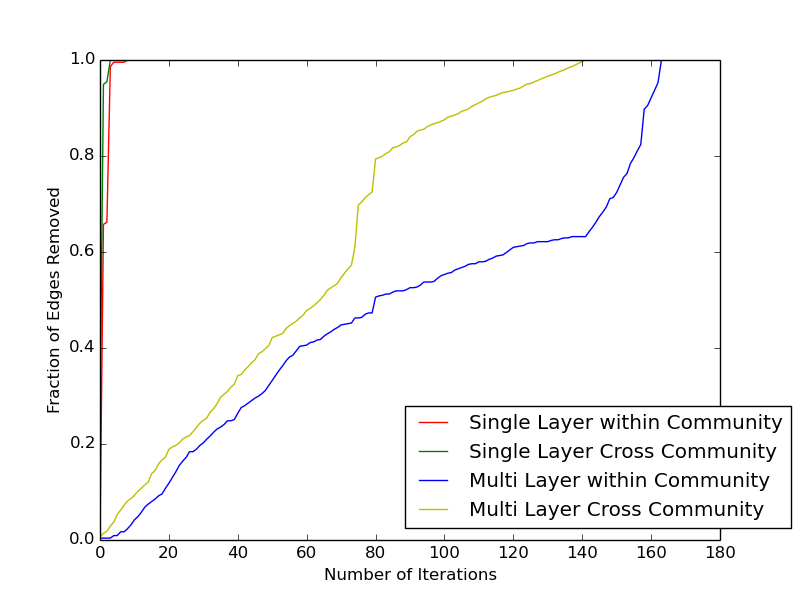
\includegraphics[angle=0,scale=.25]{./images/mp65_0_7_0_7_0_2.png}}
% \end{center}
% \vspace{-0.22in}
% \caption{CDF of different types of deleted edges while running Newman-Girvan algorithm}
% \label{d}
% \end{figure}
%
% \item \textbf{Effect of $alpha$ on NMI:} We generally find that NMI of obtained and ground truth communities decay with increasing
%  $\alpha$ (see Fig.~\ref{nmi}) irrespective of $p$ values. \textcolor{red}{[SP: It is little difficult to explain because for
%  same $p$ value ($p$=0.9), we find in Fig.~\ref{Q1} that modularity of the obtained communities increase with $\alpha$. There can be
%  two different possible reasons - a) The algorithm is obtaining better communities but different ones from the ground truth communities.
%  The Newman-Girvan algorithm treats the entire network as a single layer network and possibly finds quite the same single layer
%  communities for different $p$ and $\alpha$ values. But increasing $\alpha$, increases the fraction of multilayer communities in ground
%  truth which in turn decreases their NMI with the obtained communities. b) The second possible reason is that the
%  fraction of singleton communities generally increases with decreasing $\alpha$ and higher fraction of singleton communities improves
%  NMI.]}\\
%  \item \textbf{Effect of mixing parameter $\mu$ of LFR on the sequence of deletion of different types of edges:} In Fig.~\ref{d}, we
%  show the sequence of deletion of 4 types of edges while running the Newman-Girvan algorithm for mixing parameter $\mu = 0.05~\&~0.65$.
%  The four types of edges are - single layer within community \& cross community edges, within community \& cross community coupling edges.
%  As we know, $\mu$ is basically fraction of cross community edges for single layer LFR communities. If $\mu$ is high, the algorithm
%  automatically deletes the within community single layer edges and obtain poor communities.
%
% \end{enumerate}
